\section{Progettazione}

\subsection{Obiettivi}
Nello sviluppo del sito il gruppo si è imposto il conseguimento dei seguenti obiettivi:
\begin{itemize}
	\item Separazione tra struttura/contenuto, presentazione e comportamento per ottenere:
	\begin{itemize}
		\item Una migliore manutenibilità del sito;
		\item Un minor peso complessivo del sito e di conseguenza un miglior posizionamento sui motori
		di ricerca.
	\end{itemize}
	A tale scopo si è deciso di separare il sito nel seguente modo:
	\begin{itemize}
		\item Struttura e contenuto: le informazioni sono codificate in pagine HTML;
		\item Presentazione: si è data un'impostazione grafica al sito tramite fogli di stile CSS;
		\item Comportamento:
		\begin{itemize}
			\item Lato client: script JavaScript;
			\item Lato server: script PHP.
		\end{itemize}
	\end{itemize}
	\item Accessibilità, ossia il sito deve poter essere navigabile dal maggior numero di utenti
	possibile, compresi quelli con disabilità visive e/o motorie. Deve essere garantita indipendentemente
	dal dispositivo utilizzato;
	\item Flessibilità, cioè il sito deve poter essere consultabile da varie tipologie di dispositivi.
	In particolare è essenziale garantire all'utente la possibilità di svolgere tutte le operazioni da
	smartphone, al fine di rendere l'esperienza utente più agevole possibile.
\end{itemize}

\subsection{Layout}
Il layout del sito si contraddistingue innanzitutto per la presenza di un header, che è sempre ancorato
sul lato superiore della finestra in modo da avere i link principali sempre a portata di mano, e di un
footer collocato alla fine di ogni pagina.\\
\\
Il corpo principale della maggior parte delle pagine è invece stato pensato come un insieme di
container dove ognuno di essi corrisponde ad una sezione della pagina, e sono caratterizzati da un titolo
e da un'insieme di subcontainer che sarebbero il contenuto di quella sezione.\\
\\
Siccome la maggior parte delle unità di misura di grandezza utilizzate sono relative, l'interfaccia scala
a seconda della dimensione del font impostata.\\
\\
Rispetto allo schermo di un computer, oltre ad essere più piccolo lo schermo di uno smartphone è
fatto per essere utilizzato in modalità potrait piuttosto che in modalità landscape. Occorre quindi che
il sito si adatti a queste differenze. In primo luogo, il sito in versione mobile presenta un header che
mostra oltre al logo della pizzeria esclusivamente un'icona ad hamburger al cui click sarà possibile
mostrare/nascondere l'elenco delle voci. Inoltre, a causa dello spazio ridotto, il titolo di un
container in modalità mobile viene spostato in alto.

\newpage
\subsection{Accessibilità}
Si è prestata particolare attenzione all'accessibilità del sito. A tal riguardo sono state prese le
seguenti misure:
\begin{itemize}
	\item Aggiunta di un testo alternativo alle immagini;
	\item Assegnazione di ogni parola che è contenuto alla sua lingua di appartenenza;
	\item Utilizzo di uno schema di colori che abbiano un buon livello di contrasto tra di loro;
	\item Utilizzo di un font chiaro e semplice;
	\item Aggiunta di un \textit{breadcrumb} che indicichi la posizione attuale all'interno del sito per
	evitare il disorientamento dell'utente;
	\item Utilizzo di una struttura del sito poco profonda in modo che ogni pagina sia raggiungibile
	partendo da quella principale con non più di tre click;
	\item Come richiesto dalle \textit{WCAG}, utilizzo di due colori diversi per i link visitati e non;
	\item Adozione di un design del sito web responsive, ossia che si adatti elegantemente
	al dispositivo utilizzato.
\end{itemize}
\begin{figure}[H]
	\centering
	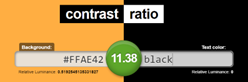
\includegraphics[scale=1]{resources/contrast_1.png}
	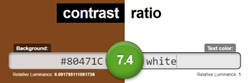
\includegraphics[scale=1]{resources/contrast_2.png}
	\caption{Livello di contrasto tra i colori di background e del font}
\end{figure}